\documentclass[11pt, a4paper]{article}
\usepackage{pdfpages}
\usepackage{parallel}
\usepackage[T2A]{fontenc}
\usepackage{ucs}
\usepackage[utf8x]{inputenc}
\usepackage[polish,english,russian]{babel}
\usepackage{hyperref}
\usepackage{rotating}
\usepackage[inner=2cm,top=1.8cm,outer=2cm,bottom=2.3cm,nohead]{geometry}
\usepackage{listings}
\usepackage{graphicx}
\usepackage{wrapfig}
\usepackage{longtable}
\usepackage{indentfirst}
\usepackage{array}
\usepackage{tikzsymbols}
\usepackage{soul}
\usepackage[ruled,vlined]{algorithm2e}
%\counterwithout{figure}{section} 

\usepackage{url}
\makeatletter
\g@addto@macro{\UrlBreaks}{\UrlOrds}
\makeatother

\newcolumntype{P}[1]{>{\raggedright\arraybackslash}p{#1}}
\frenchspacing
\usepackage{fixltx2e} %text sub- and superscripts
\usepackage{icomma} % коскі ў матэматычным рэжыме
\PreloadUnicodePage{4}

\newcommand{\longpage}{\enlargethispage{\baselineskip}}
\newcommand{\shortpage}{\enlargethispage{-\baselineskip}}

\def\switchlang#1{\expandafter\csname switchlang#1\endcsname}
\def\switchlangbe{
\let\saverefname=\refname%
\def\refname{Літаратура}%
\def\figurename{Іл.}%
}
\def\switchlangen{
\let\saverefname=\refname%
\def\refname{References}%
\def\figurename{Fig.}%
}
\def\switchlangru{
\let\saverefname=\refname%
\let\savefigurename=\figurename%
\def\refname{Литература}%
\def\figurename{Рис.}%
}

\hyphenation{admi-ni-stra-tive}
\hyphenation{ex-pe-ri-ence}
\hyphenation{fle-xi-bi-li-ty}
\hyphenation{Py-thon}
\hyphenation{ma-the-ma-ti-cal}
\hyphenation{re-ported}
\hyphenation{imp-le-menta-tions}
\hyphenation{pro-vides}
\hyphenation{en-gi-neering}
\hyphenation{com-pa-ti-bi-li-ty}
\hyphenation{im-pos-sible}
\hyphenation{desk-top}
\hyphenation{elec-tro-nic}
\hyphenation{com-pa-ny}
\hyphenation{de-ve-lop-ment}
\hyphenation{de-ve-loping}
\hyphenation{de-ve-lop}
\hyphenation{da-ta-ba-se}
\hyphenation{plat-forms}
\hyphenation{or-ga-ni-za-tion}
\hyphenation{pro-gramming}
\hyphenation{in-stru-ments}
\hyphenation{Li-nux}
\hyphenation{sour-ce}
\hyphenation{en-vi-ron-ment}
\hyphenation{Te-le-pathy}
\hyphenation{Li-nux-ov-ka}
\hyphenation{Open-BSD}
\hyphenation{Free-BSD}
\hyphenation{men-ti-on-ed}
\hyphenation{app-li-ca-tion}

\def\progref!#1!{\texttt{#1}}
\renewcommand{\arraystretch}{2} %Іначай формулы ў матрыцы зліпаюцца з лініямі
\usepackage{array}

\def\interview #1 (#2), #3, #4, #5\par{

\section[#1, #3, #4]{#1 -- #3, #4}
\def\qname{LVEE}
\def\aname{#1}
\def\q ##1\par{{\noindent \bf \qname: ##1 }\par}
\def\a{{\noindent \bf \aname: } \def\qname{L}\def\aname{#2}}
}

\def\interview* #1 (#2), #3, #4, #5\par{

\section*{#1\\{\small\rm #3, #4. #5}}
\ifx\ParallelWhichBox\undefined%
    \addcontentsline{toc}{section}{#1, #3, #4}%
\else%
\ifnum\ParallelWhichBox=0%
    \addcontentsline{toc}{section}{#1, #3, #4}%
\fi\fi%

\def\qname{LVEE}
\def\aname{#1}
\def\q ##1\par{{\noindent \bf \qname: ##1 }\par}
\def\a{{\noindent \bf \aname: } \def\qname{L}\def\aname{#2}}
}

\newcommand{\interviewfooter}[1]{
\vskip 1em
\noindent \textit{#1}
}

\switchlang{ru}
\begin{document}

\title{1996 "--- Q500 mouse}
\date{}
\maketitle
\selectlanguage{russian}
    Q500 mouse (рис. \ref{fig:q500mousePic}) выпускалась в Южной Корее и была (наряду с Hi-Bon Optical laser mouse LMOX-2) одной из двух необычных оптических мышей, разработанных в 1996 году iO TEK и использующих в своей конструкции световоды. Вероятно, Q500 mouse обладает рекордно дешевой конструкцией оптических мышей из когда-либо изобретенных.

\begin{figure}[h]
    \centering
    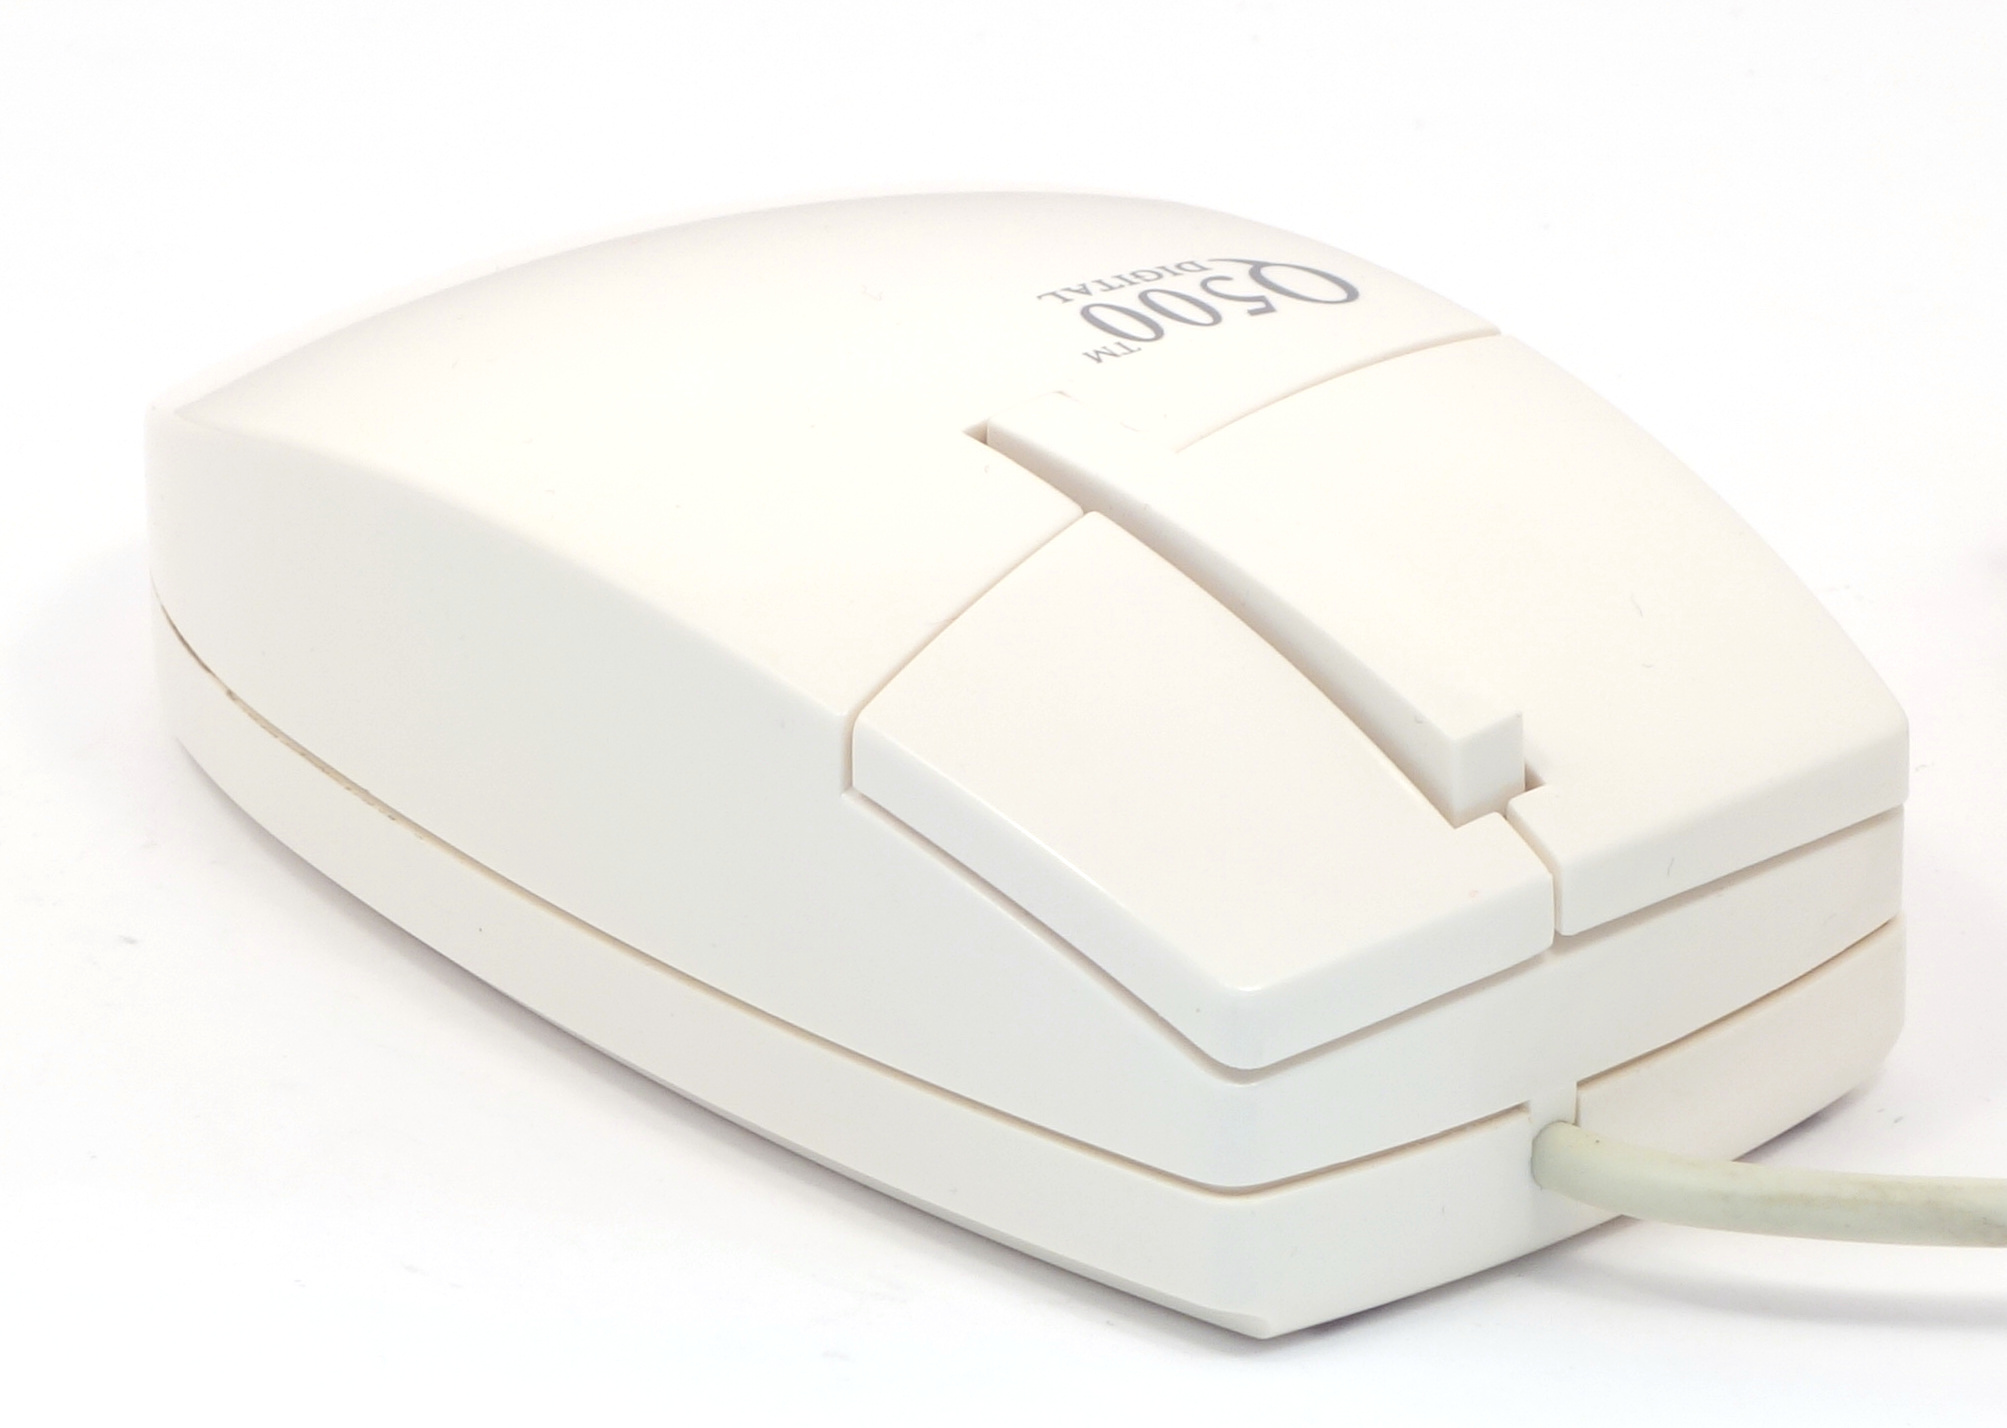
\includegraphics[scale=0.5]{1996_q500_mouse/pic_30.jpg}
    \caption{Q500 mouse}
    \label{fig:q500mousePic}
\end{figure}

Как в случае абсолютного большинства ранних оптических мышей, данному манипулятору требуется коврик с отражающей сеткой (рис. \ref{fig:q500mousePad}). В отличие от металлических ковриков Mouse Systems с решеткой из вертикальных и горизонтальных линий, соответствующих двум разным длинам волн, здесь применяются светлая поверхность и одноцветные темные линии (рис. \ref{fig:q500mousePad}). Как можно заметить, используется два блока (блок горизонтальных линий и блок вертикальных), каждый из которых занимает половину коврика.



\begin{figure}[h]
    \centering
    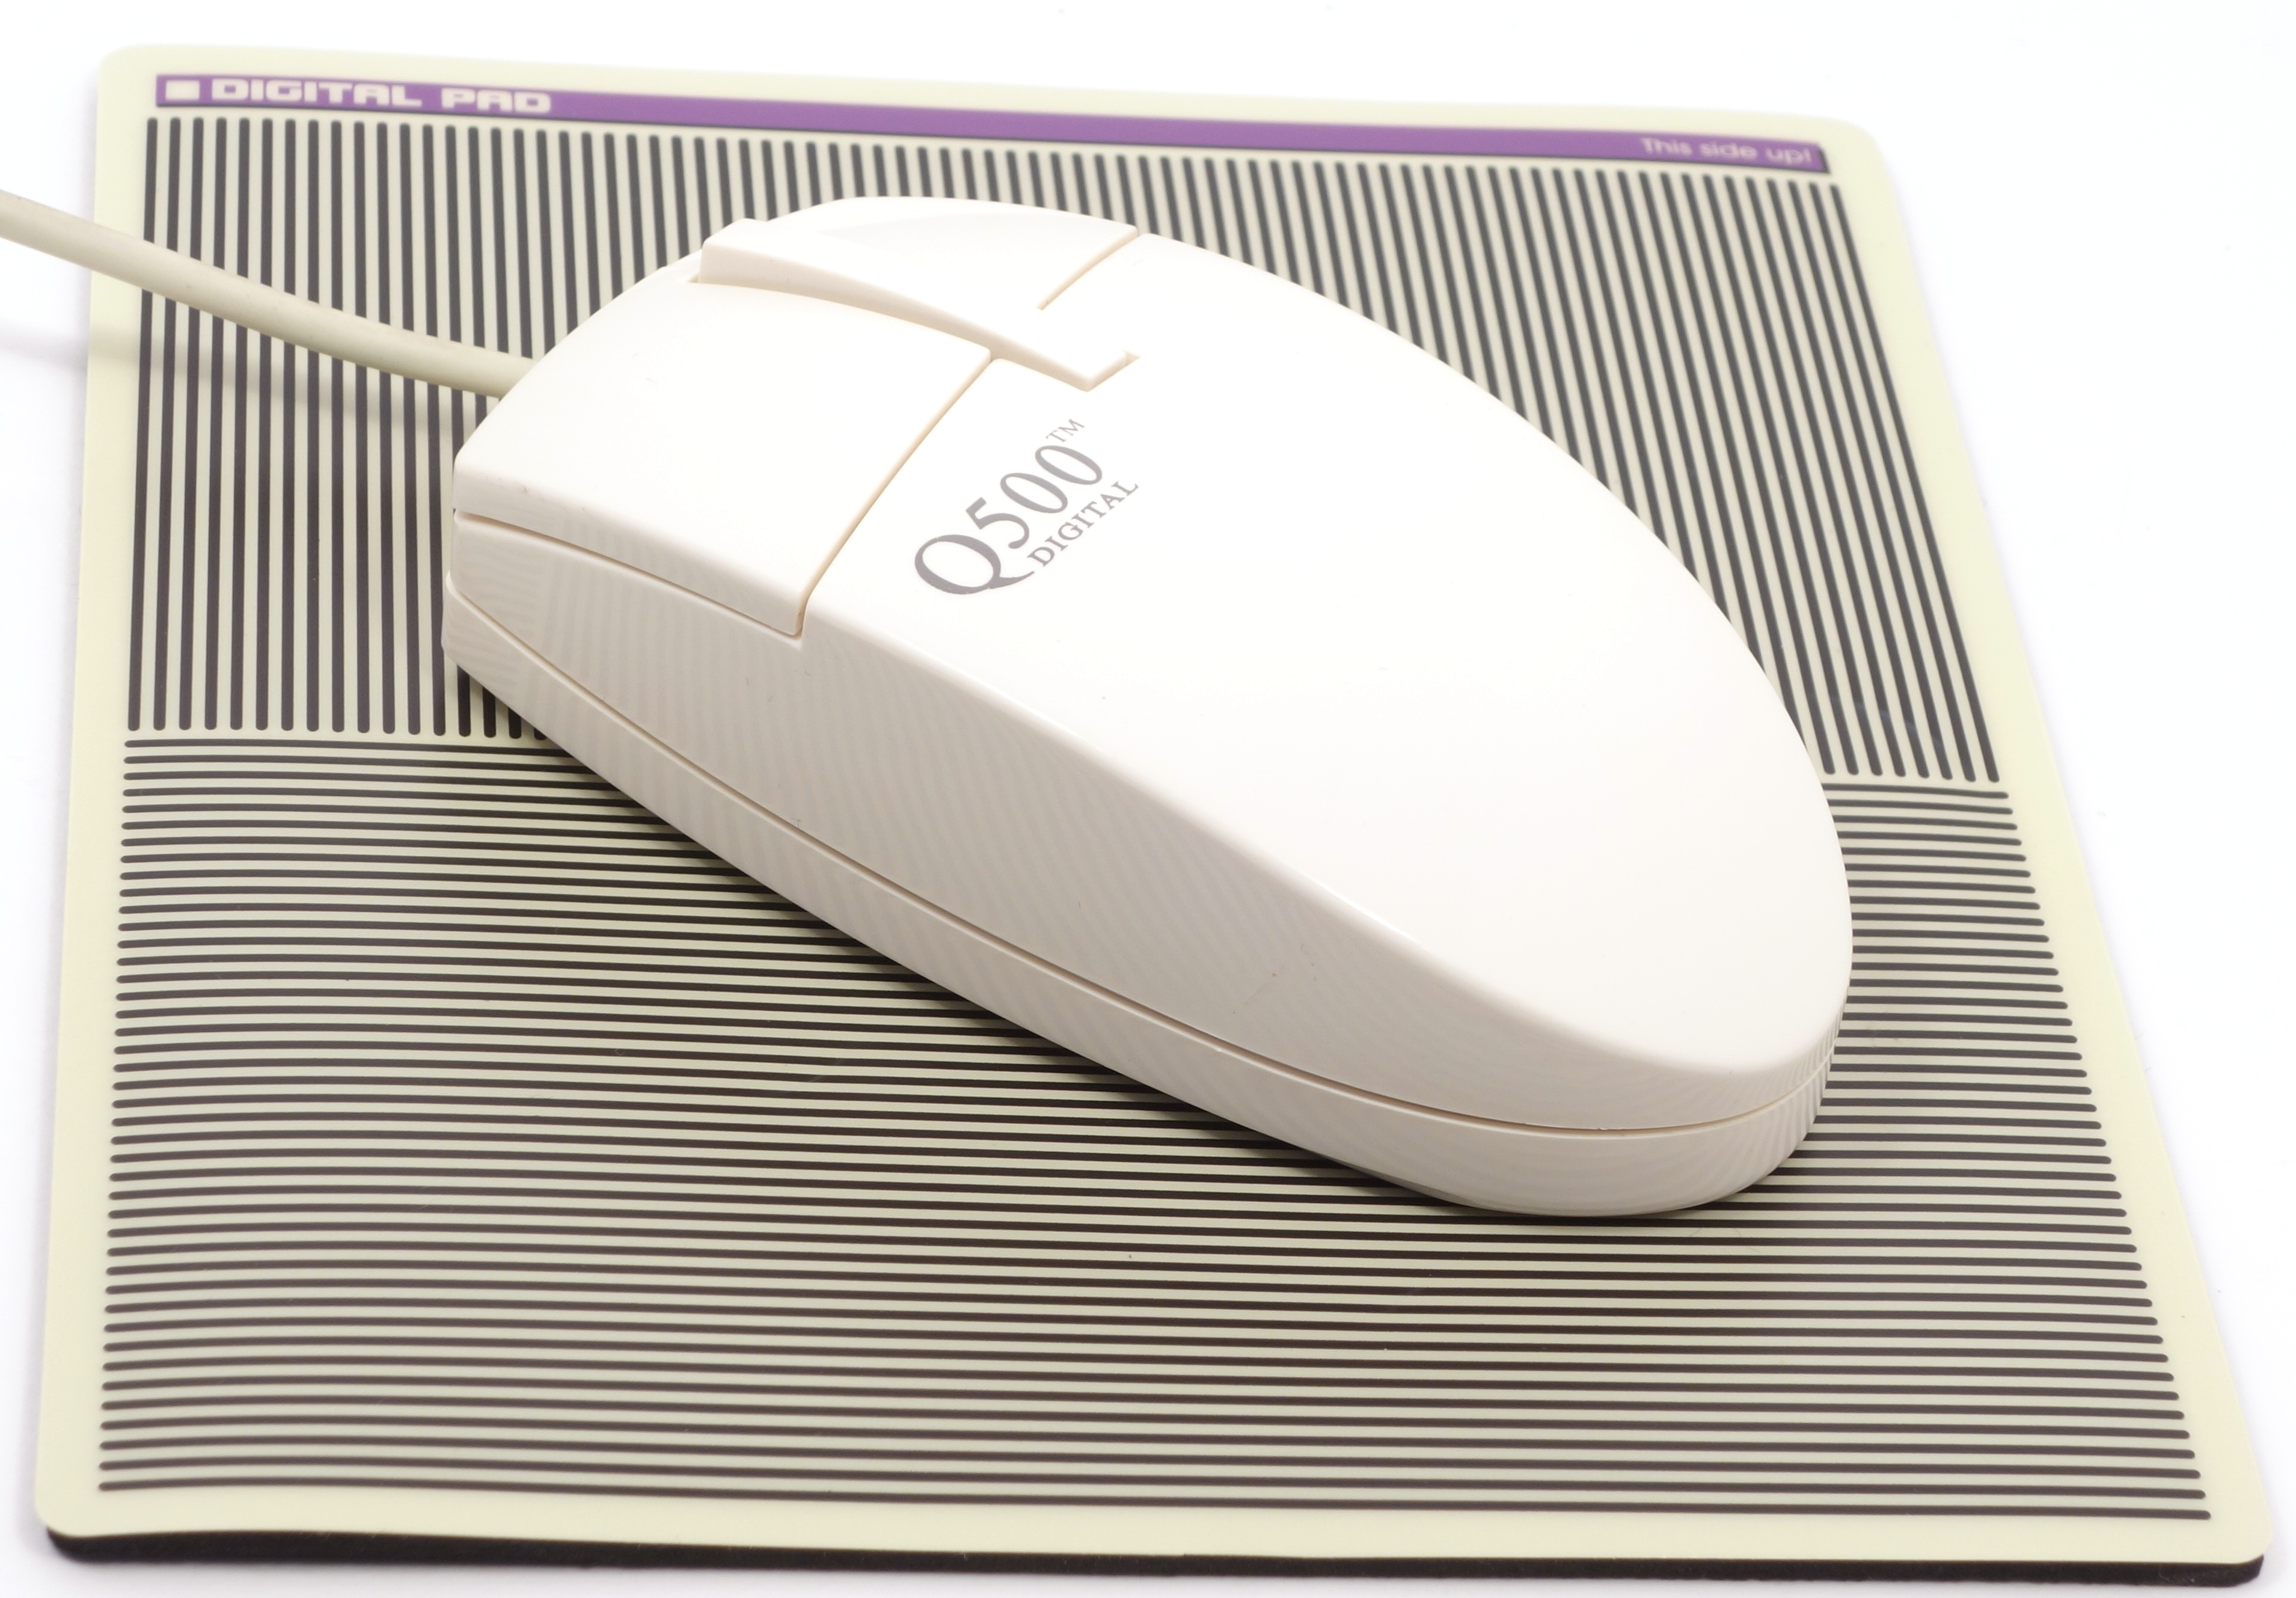
\includegraphics[scale=0.4]{1996_q500_mouse/pad_30.jpg}
    \caption{Q500 mouse на комплектном коврике}
    \label{fig:q500mousePad}
\end{figure}

Малый размер коврика объясняется тем, что с каждому из двух датчиков мыши соответствует свой блок полос.
При этом два датчика мыши расположены в корпусе максимально далеко друг от друга (рис. \ref{fig:q500mouseTopBottom}) для того, чтобы они не могли потерять соответствующие участки, даже если переместить мышь к самому краю коврика. Поэтому увеличение коврика потребовало бы аналогичного увеличения размеров мыши.

Конструкция Q500 по существу является модификацией стандартной оптомеханической мыши на базе пары поворотных энкодеров: в случае Q500 прорези на дисках энкодеров <<развернуты>> в блок линий на коврике, и таким обрзаом поворотные энкодеры заменены линейными. Это сходство делает возможным использование в Q500 микросхемы-контроллера любой опто-механической мыши, упрощая выбор элементной базы \cite{yq}.

\begin{figure}[h]
    \centering
    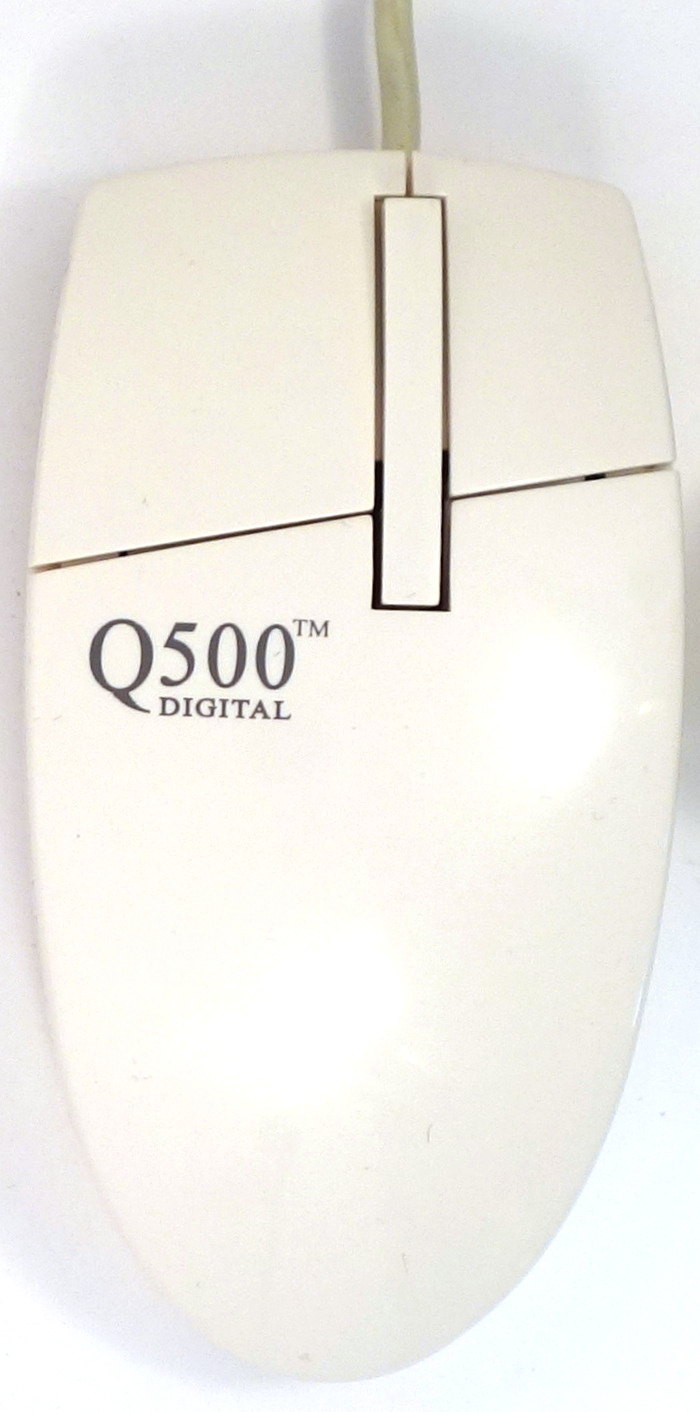
\includegraphics[scale=0.5]{1996_q500_mouse/top_30.jpg}
    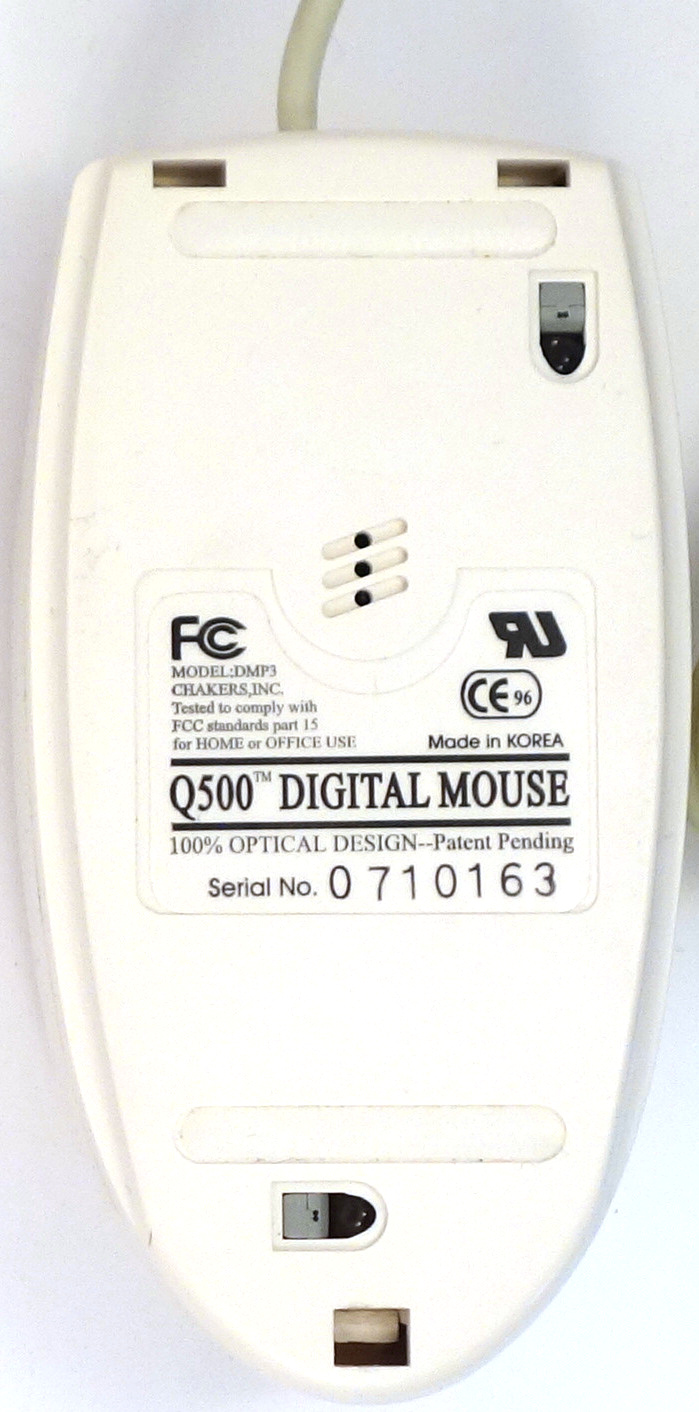
\includegraphics[scale=0.5]{1996_q500_mouse/bottom_30.jpg}
    \caption{Q500 mouse, вид сверху и снизу}
    \label{fig:q500mouseTopBottom}
\end{figure}

По размеру и форме мышь является типичным манипулятором 90-х годов (рис. \ref{fig:q500mouseSize}).

\begin{figure}[h]
    \centering
    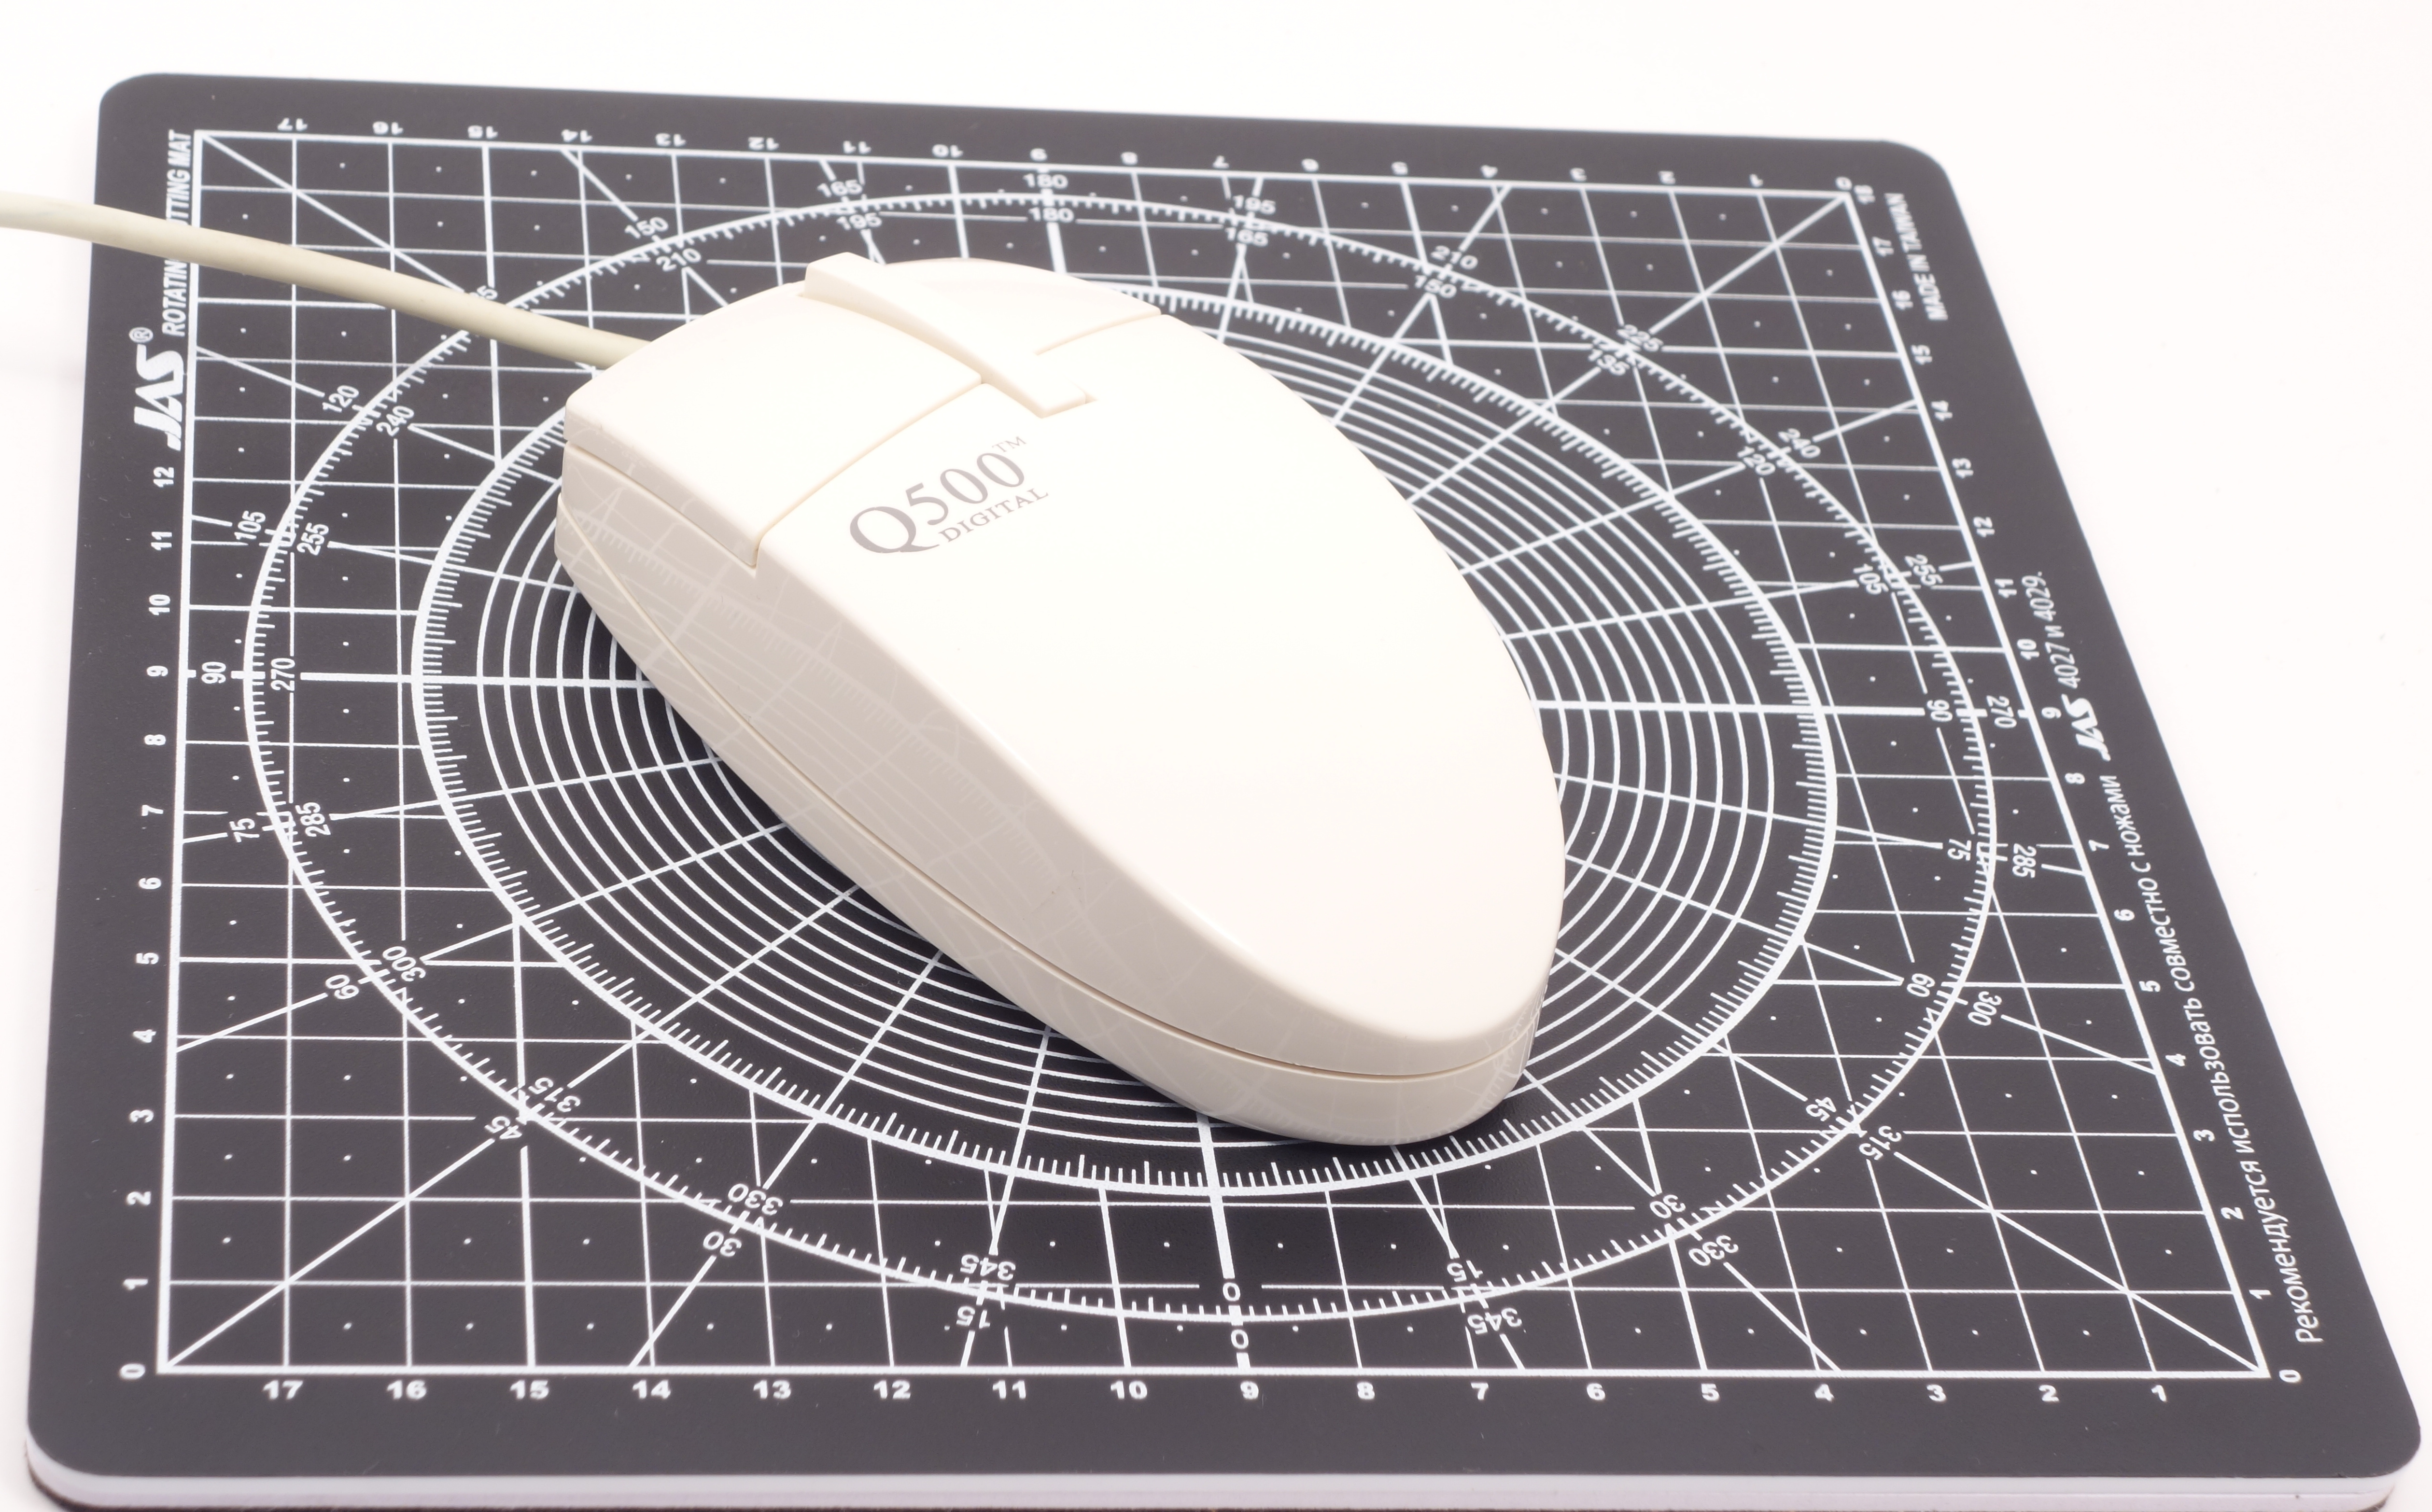
\includegraphics[scale=0.25]{1996_q500_mouse/size.jpg}
    \caption{Q500 mouse на размерном коврике с шагом сетки 1~см}
    \label{fig:q500mouseSize}
\end{figure}

Мышь имеет достаточно удобные левую и правую кнопки (рис. \ref{fig:q500mouseHand}), а также третью узкую кнопку, форма которой подсказывает, что она едва ли предназначена для частых нажатий.

\begin{figure}[h]
    \centering
    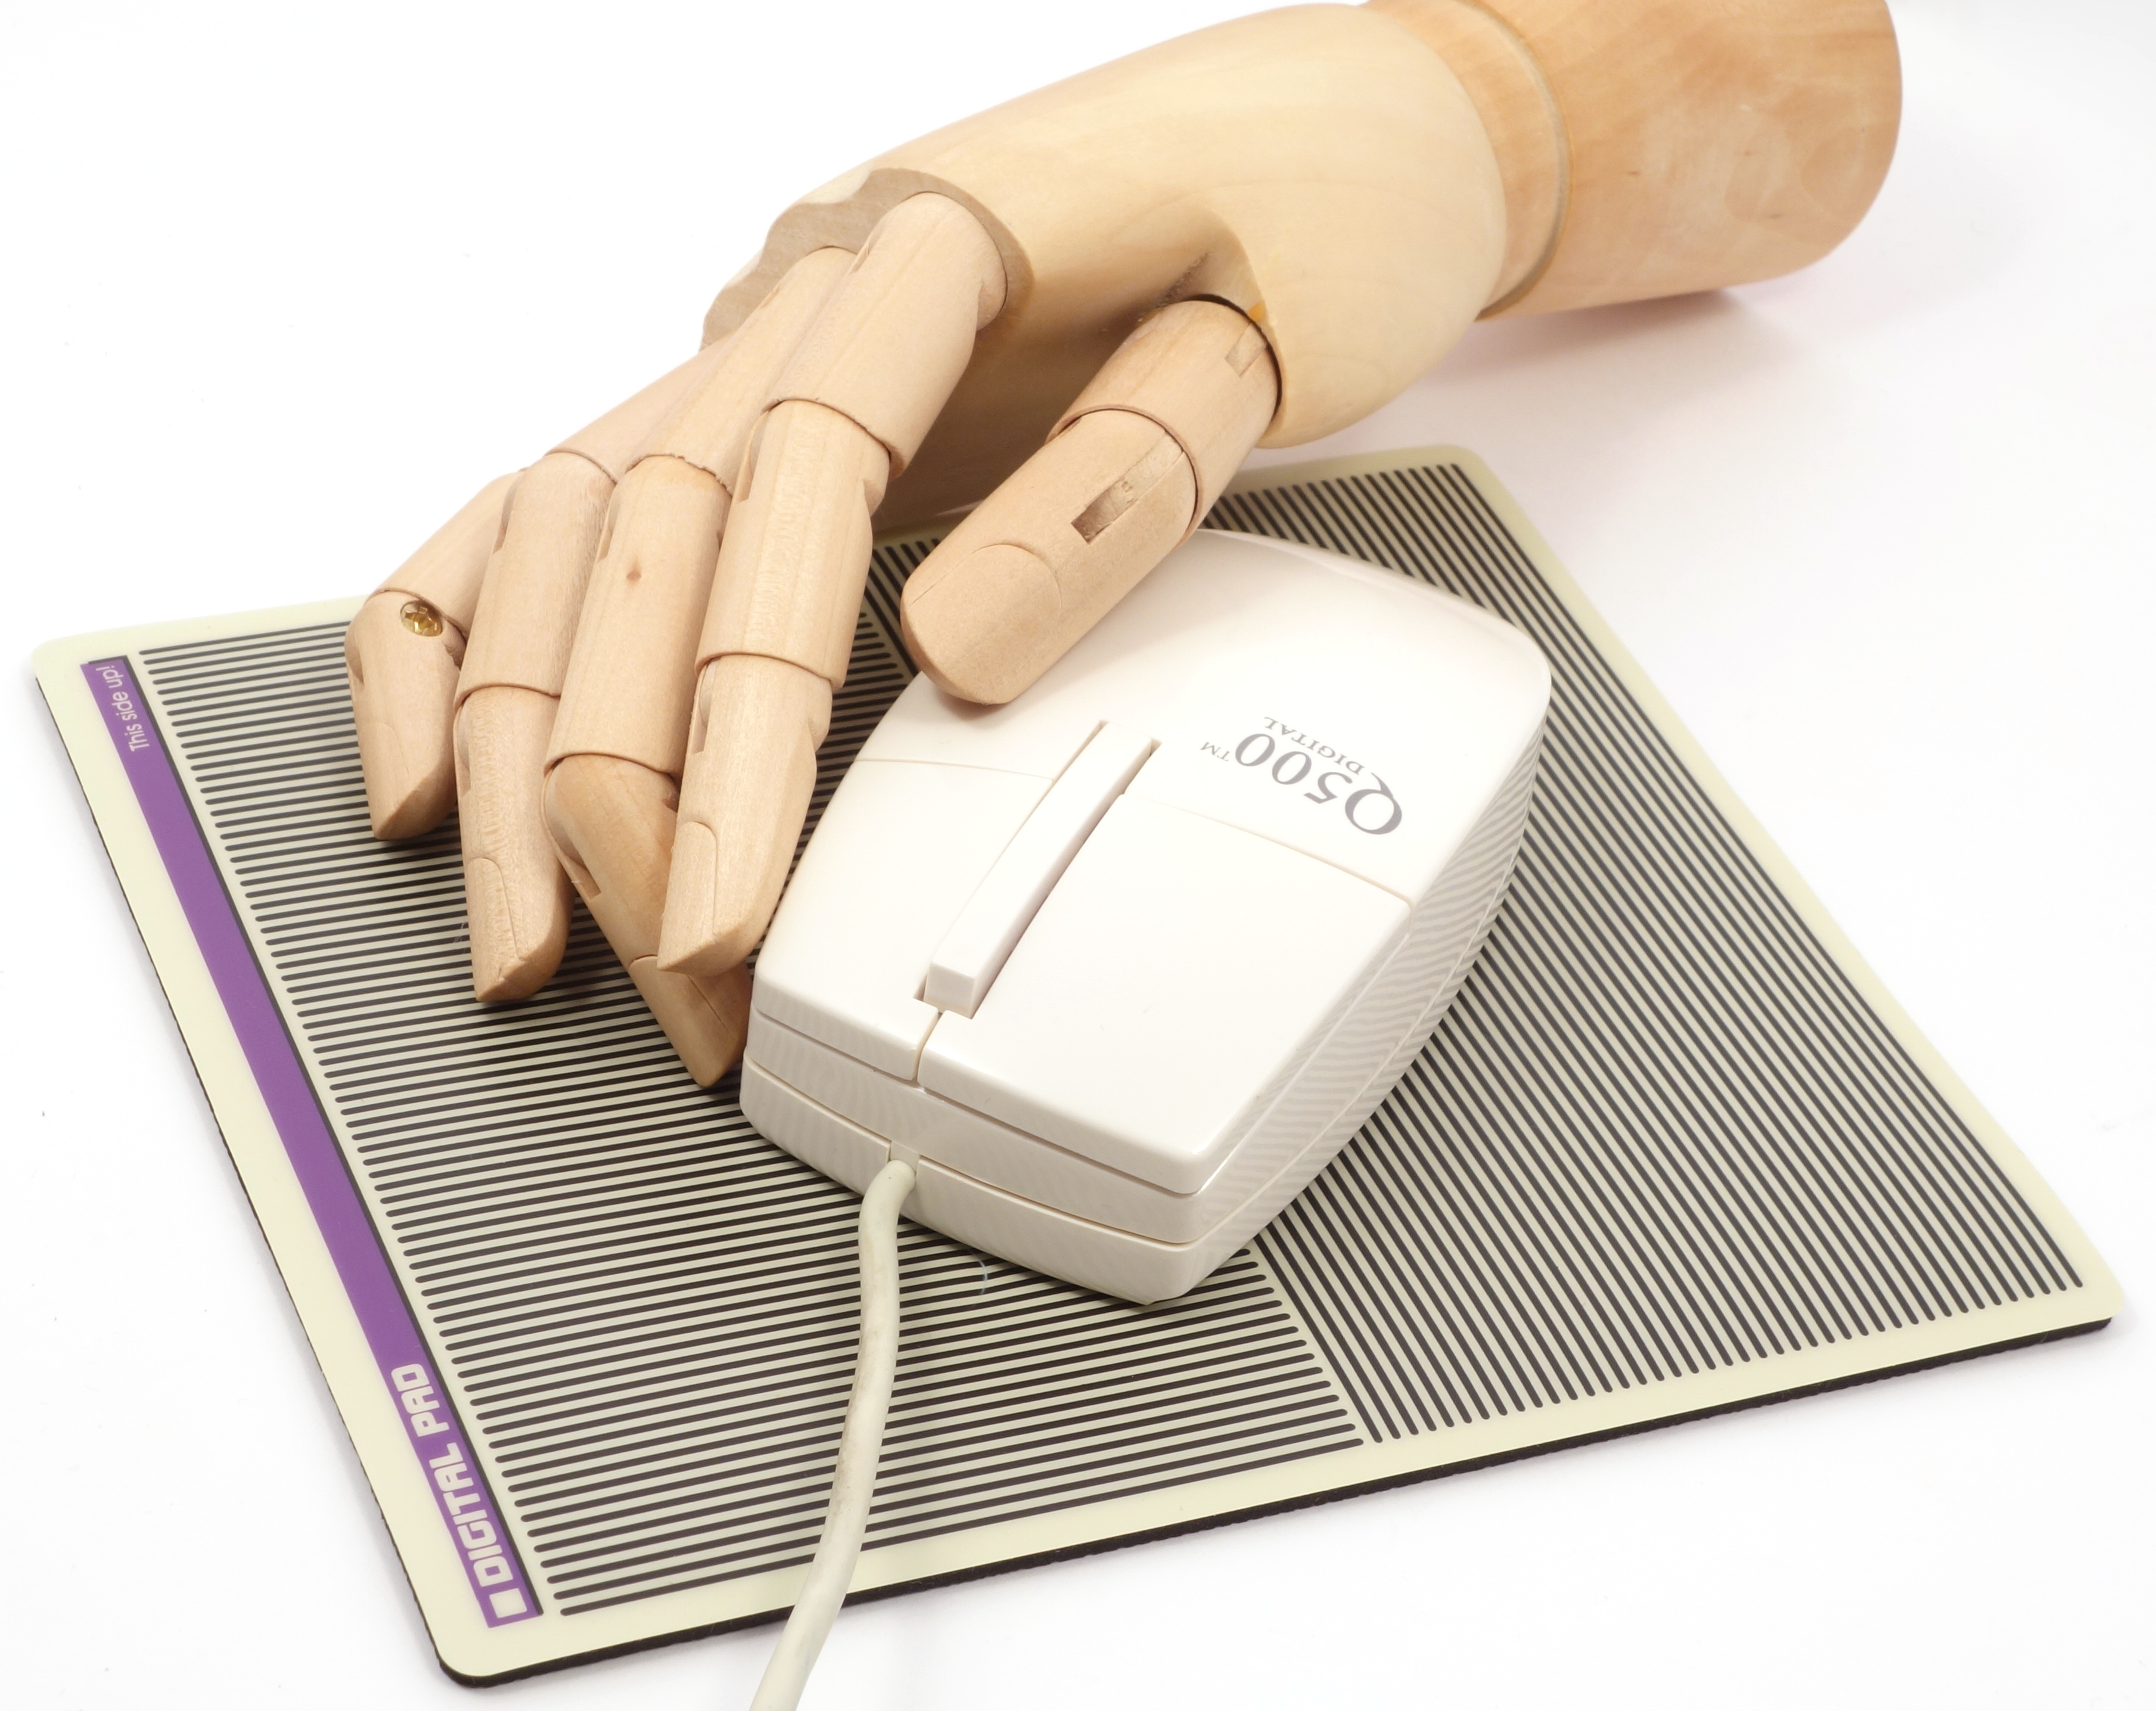
\includegraphics[scale=0.4]{1996_q500_mouse/hand_30.jpg}
    \caption{Q500 с моделью руки человека}
    \label{fig:q500mouseHand}
\end{figure}


Внутреннее устройство показано на рис. \ref{fig:q500mouseInside}.
Половинки корпуса соединяются защёлками, без винтов. Монолитный блок в центре, куда входят световоды, скрывает в себе два фотодиода. В отличие от мышей Mouse Systems, использующих отдельные датчики для каждой оси, 
конструкция Q500 дополнительно удешевлена тем, что светодиоды включаются поочерёдно, чтобы фотодиоды сначала получали выборку по горизонтали, а затем по вертикали \cite{yq}.

\begin{figure}[h]
    \centering
    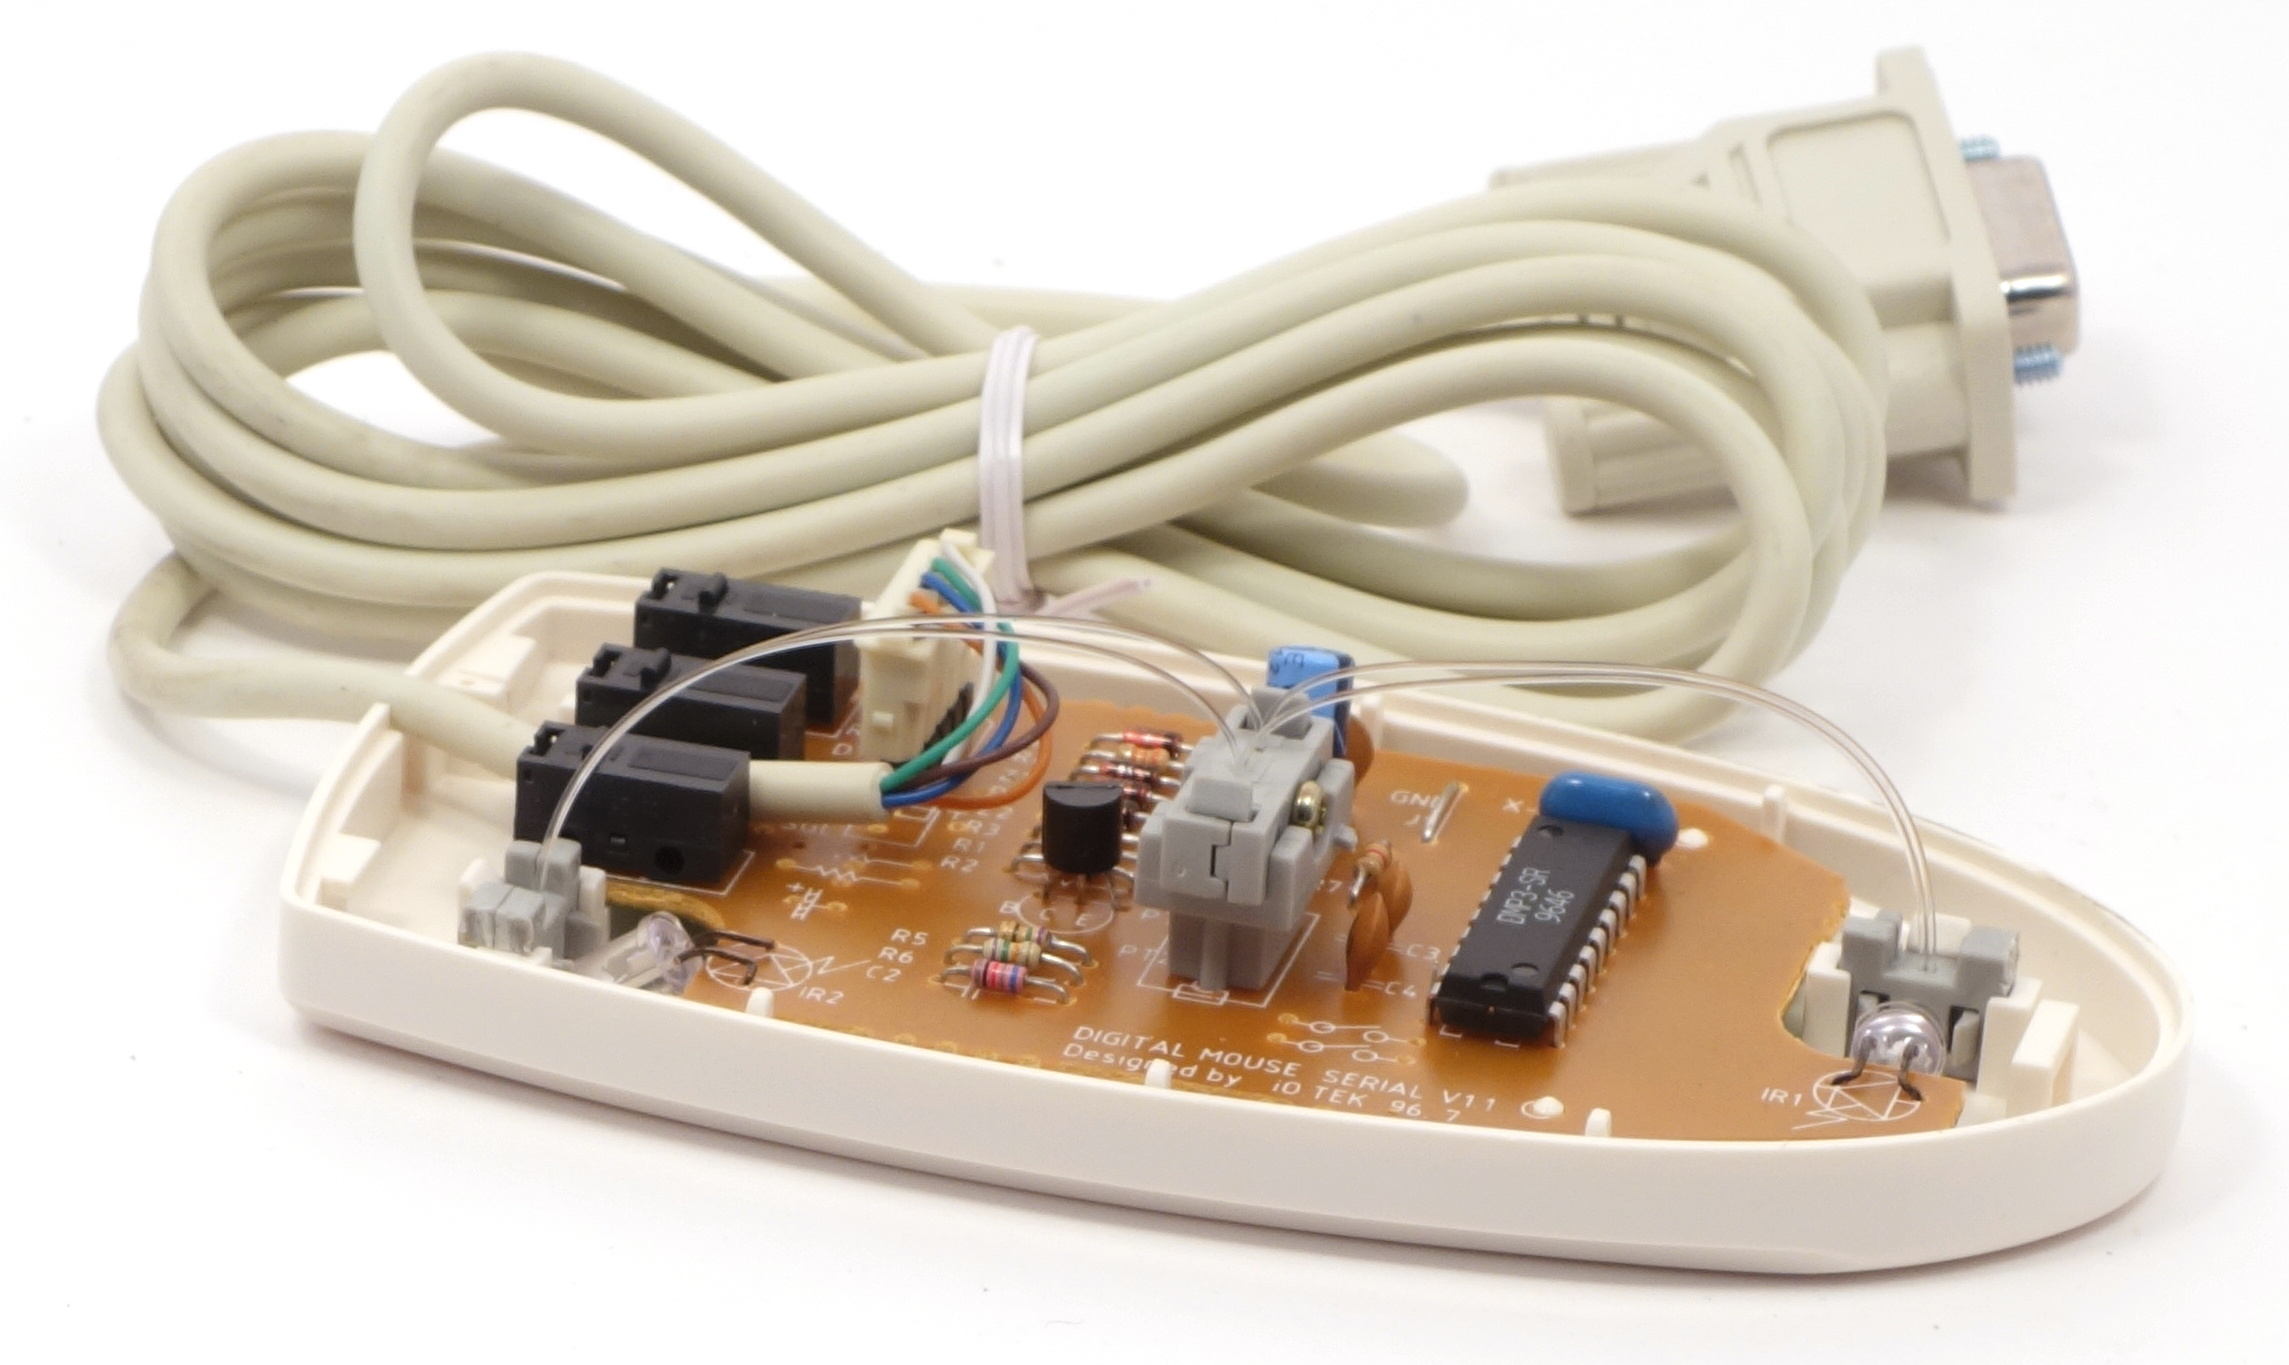
\includegraphics[scale=0.8]{1996_q500_mouse/inside_30.jpg}
    \caption{Q500 mouse в разобранном виде}
    \label{fig:q500mouseInside}
\end{figure}

Надпись на печатной плате показывает, что данная мышь была, как и Hi-Bon Optical laser mouse, разработана на контрактной основе компанией iO TEK в 1996 году.

При этом, согласно видеообзору, приведенному в \cite{yq}, на практике мышь перемещает курсор лишь чуть грубее, чем обычная мышь. Единственная реальная проблема заключается в том, что если коврик не должен быть повернут относительно мыши (даже слегка). Также, если край мыши (и соответственно один из датчиков) выходит за пределы коврика, мышь теряет способность регистрировать перемещения по соответствующей оси.

\begin{thebibliography}{9}
\bibitem {yq} Q500, The Weirdest Optical Mouse \url{https://www.youtube.com/watch?v=Cd6lxwjX2Bk}
\end{thebibliography}
\end{document}
